\documentclass[9pt]{beamer}
\usetheme[block=fill]{metropolis}
%\setbeamersize{text margin left=.2cm,text margin right=.2cm}

\usepackage{amsthm}
\usepackage{amsmath}
\usepackage{amsfonts}
\usepackage{amssymb}

\usepackage{graphicx}
\graphicspath{{../../images/}}
%\usepackage[french]{babel}
%\usepackage{listings}
%\usepackage{lipsum}
\usepackage{boolexpr}
\usepackage{kpfonts}
\usepackage{caption}
\usepackage{wrapfig}
%\usepackage{chngcntr}
\usepackage[labelformat=empty]{caption}
\usepackage[official]{eurosym}

\newcommand{\induced}{\rho}
\newcommand{\induceda}{\induced^{(1)}}
\newcommand{\inducedb}{\induced^{(2)}}

%\newcommand{\gatpar}{Gatermann, Parrilo, \emph{{S}ymmetry groups, semidefinite programs, and sums of squares}, Journal of Pure and Applied Algebra, 2004}
\newcommand{\gatpar}{Gatermann, Parrilo, \emph{{S}ymmetry groups, semidefinite programs, and sums of squares}, 2004}
\newcommand{\citefoot}[1]{\footnote{\tiny #1}}

\usepackage{minted}

\usepackage{siunitx}

% http://tex.stackexchange.com/questions/114830/how-can-i-use-lvert-and-rvert-norm-symbols-x-with-the-iwona-math-font
% \usepackage[math]{iwona}
% \usepackage{scalerel}
\def\lVert{\mid\!\mid}
\def\rVert{\mid\!\mid}

\usepackage[sfdefault, lf, light, semibold]{FiraSans}
% \usepackage[]{lucbmath}
\usepackage{bbm}
\usepackage[T1]{fontenc}


\usepackage[normalem]{ulem}
%\newcommand{\Adj}{\mathbf{A}}
\usepackage{mathtools}

\usepackage{../../custom}
\usepackage{amsfonts}
\usepackage{amsmath}
\usepackage{amsthm}
%\newcommand{\jsrcodepath}{../../code}
%\usepackage{jsr}

\newcommand{\expe}[2]{\la #1, #2 \ra}

\usepackage{framed}

%\usepackage{mathtools,xparse}
%\DeclarePairedDelimiter{\norm}{\lVert}{\rVert}
\newcommand\Wider[2][3em]{%
\makebox[\linewidth][c]{%
  \begin{minipage}{\dimexpr\textwidth+#1\relax}
  \raggedright#2
  \end{minipage}%
  }%
}

\newcommand{\aeur}{\alpha_\text{\euro}}
\newcommand{\adol}{\alpha_\$}
\newcommand{\apou}{\alpha_\text{\pounds}}

% footnote without number: \footnote[]{some text}
% source: https://tex.stackexchange.com/questions/170511/footnotes-without-numbering
\let\svthefootnote\thefootnote
\textheight 1in
\newcommand\blankfootnote[1]{%
  \let\thefootnote\relax\footnotetext{#1}%
  \let\thefootnote\svthefootnote%
}
\let\svfootnote\footnote
\renewcommand\footnote[2][?]{%
  \if\relax#1\relax%
    \blankfootnote{#2}%
  \else%
    \if?#1\svfootnote{#2}\else\svfootnote[#1]{#2}\fi%
  \fi
}

\newcommand{\comment}[1]{\noindent 
\begin{footnotesize}
{\color{black!40} #1}
\end{footnotesize}
}

\title{Positivity, symmetry and semi-definite optimization}
\date{Poznań}
\author{
Marek Kaluba \tiny KIT, Karlsruhe, Germany \normalsize}
\institute{Introduction to Computational Mathematics 2022}

% https://tex.stackexchange.com/questions/426088/texlive-pretest-2018-beamer-and-subfig-collide
\makeatletter
\let\@@magyar@captionfix\relax
\makeatother
\begin{document}
  \maketitle

  \begin{frame}{Group Theory to the rescue!}
  \begin{block}{Definition}
    A \alert{group} $(G, *)$ is a set closed under the multiplication $*$, together with the existence of unique inverse elements.
  \end{block}
    {\small Example: The set of all bijections of the set $\{1,\ldots n\}$ with composition is a group (known as the full symmetric group on $n$ letters $S_n$).}

    $S_2 = \{(1)(2), (1,2)\}$ \alert{acts} on polynomial ring $\mathbb{R}[x]$ by
    \begin{align*}
      ((1)(2), x) & \mapsto x\\
      ((1, 2), x) & \mapsto -x.
    \end{align*}
    {\small 
%     Observe: $f(x) = x^4 - 2x^2$ is invariant under this action.\\
    Observe: $f(x) = x^6 - 2x^4 + 2x^2 = x^2 + (x-x^3)^2$ is invariant, but $x-x^3$ isn't!}

\end{frame}


\begin{frame}{Isotypical projections}
    ``Types'' of actions $\leftrightarrow$  blocks in the block-diagonalization:
    \[V \cong V_1 \oplus \cdots \oplus V_k.\]
    Each block $V_i$ decomposes further as
    $V = \bigoplus_i \oplus_{m_i} V_i'$. (\footnote{$m_i$ is the multiplicity of the action type in $V$})

    Universal (baseless) \alert{projections}\footnote{related to irreducible characters} in group ring $\mathbb{R}[G]$ $\leftrightarrow$ projections onto blocks (for every representation $V$!).
%
    \begin{block}{Example}
    \small
    Universal \textbf{projections} for $S_2$:\\[-0.2in]
    \begin{align*}
      \pi_1 = \frac{1}{2}((1)(2) + (1,2)) & \to\text{invariants}\\
      \pi_2 = \frac{1}{2}((1)(2) - (1,2)) & \to\text{flipped}
    \end{align*}
    \end{block}

\end{frame}

\begin{frame}[fragile]{Permutation symmetry example}
\footnotesize
\begin{minted}{julia}
  using PermutationGroups
  G = PermGroup([perm"(1,2,3,4)"])
  # permutation group generated by one element (cyclic of order 4)
  using DynamicPolynomials
  @polyvar x[1:4]
  poly = sum(x) + sum(x.^2)
  basis = monomials(x, 0:(maxdegree(f)÷2))
  using SymbolicWedderburn
  symmetry_adapted_basis(G, basis, Symmetry.VariablePermutation())
  # G acts by permuting variables
\end{minted}

Isotypical blocks when acting on $[1, x_1, x_2, x_3, x_4, x_5]$:
\[
  B_1 = \begin{bmatrix}
          1\\
          x_1 + x_2 + x_3 + x_4
        \end{bmatrix}
  \qquad
  B_2 = \begin{bmatrix}
          x_1 - x_3\\
          x_2 - x_4
        \end{bmatrix}
  \qquad
  B_3 = \begin{bmatrix}
          x_1 - x_2 + x_3 - x_4
        \end{bmatrix}
\]

  \[V \cong (V_{\alert{1}}' \oplus V_{\alert{1}}') \oplus V_2' \oplus V_3', \qquad d_2 = m_1 = 2, \quad d_1 = d_3 = m_2 = m_3 = 1.\]
  %\[V \cong (V_1' \oplus V_1') \oplus V_2' \oplus V_3', \qquad m_1 = 2, \quad m_2 = m_3 = 1.\]
\end{frame}

\begin{frame}[fragile]{Permutation symmetry example}
\footnotesize
\begin{minted}{julia}
  using SumOfSquares
  import ECOS # Note: ECOS doesn't support PSD cone,
  # but 2×2 psd constraints translate to SOC/quadratic constraints
  model = Model(ECOS.Optimizer)
  @variable(model, t)
  @objective(model, Max, t)
  pattern = Symmetry.Pattern(G, Symmetry.VariablePermutation())
  @constraint(model, poly - t in SOSCone(), symmetry = pattern)
  optimize!(model)
\end{minted}

\normalsize

  Naive: 15 vars 15 constrs, $Q$ is $5\times 5$; Symmetry: 5 vars 5 constrs,
  \[ Q = Q_1 \oplus (Q_{\alert{2}} \oplus Q_{\alert{2}}) \oplus Q_3 \qquad Q_1 \text{ is }2\times 2, Q_2 \text{ is }1\times 1, Q_3 \text{ is }1\times 1 \]
  %\[ m_1 \times m_1, m_2 \times m_2, m_3 \times m_3 \qquad 2\times 2, 1\times 1, 1\times 1 \]

  Note inversion: multiplicities $\leftrightarrow$ dimensions
  \[V \cong (V_{\alert{1}}' \oplus V_{\alert{1}}') \oplus V_2' \oplus V_3', \qquad d_2 = m_1 = 2, \quad d_1 = d_3 = m_2 = m_3 = 1.\]
%Note: the sizes here correspond to the multiplicities of irreducible subspaces, \textbf{not} their dimensions!

\end{frame}

\begin{frame}[fragile]{Even symmetry example\citefoot{\gatpar{}: Example~5.1}}
\footnotesize
\begin{minted}{julia}
  struct OnSign <: Symmetry.OnMonomials end
  # <: SymbolicWedderburn.Action, corresponds to x → -x
  SymbolicWedderburn.action(::OnSign, p::Permutation,
      mono::AbstractMonomial) = sign(p)^degree(mono)*mono
  G = PermGroup([perm"(1,2)"])
  @polyvar x
  f = x^6 - 2x^4 + 2x^2
  basis = monomials(x, 0:(maxdegree(f)÷2))
  symmetry_adapted_basis(G, basis, OnSign())
\end{minted}

  Isotypical blocks when acting on $[1, x, x^2, x^3]$:
\[
  B_1 = \begin{bmatrix}
          1\\
          x^2
        \end{bmatrix}
  \qquad
  B_2 = \begin{bmatrix}
          x\\
          x^3
        \end{bmatrix}
  \qquad
  V = (V_1' \oplus V_1') \oplus (V_2' \oplus V_2')
\]

  \vspace{-1em}

Naive formulation $4\times 4$-psd; with symmetry: $2\times 2$, $2\times 2$-psd.
\end{frame}

\begin{frame}[fragile]{Dihedral symmetry example\citefoot{\gatpar{}: Example~5.4}}
\footnotesize
  \begin{minted}{julia}
  @polyvar x y
  f = x^6 + y^6 - x^4 * y^2 - y^4 * x^2 - x^4 - y^4 -
      x^2 - y^2 + 3x^2 * y^2 + 1
  struct DihedralAction <:
      SymbolicWedderburn.ByLinearTransformation end
  \end{minted}
  The action is a mixture of changing sign and permuting variables.

  \vspace{-2em}

  \begin{align*}
    B_1 = [x^2 + y^2, 1], & \qquad m_1 = 2, d_1 = 1,\\
    B_2 = [x^3, x^2y, xy^2, y^3, x, y], & \qquad m_2 = 3, d_2 = 2,\\
    B_3 = [xy], & \qquad m_3 = d_3 = 1,\\
    B_4 = [x^2 - y^2], & \qquad m_4 = d_4 = 1,
  \end{align*}

  \vspace{-1em}

  $10 \times 10$-psd into $2 \times 2$, $3 \times 3$, $1 \times 1$, $1 \times 1$-psd.

  \vspace{-1em}

  \alert{Non}-commutative groups allow $d_i > 1$ $\to$ \alert{better} for the symmetrization!
\end{frame}

\begin{frame}[fragile]{Implementing group action}
\footnotesize

  \begin{minted}{julia}
  import GroupsCore
  struct DihedralGroup <: GroupsCore.Group ... end
  struct DihedralElement <: GroupsCore.GroupElement
      ...
  end
  \end{minted}
\normalsize
  \begin{itemize}
    \item implement methods from \texttt{GroupsCore.jl} API for \texttt{DihedralGroup}
    \item implement action methods from \texttt{SymbolicWedderburn} for \texttt{DihedralAction}
  \end{itemize}
\end{frame}

\begin{frame}{Behind the scenes: \texttt{SymbolicWedderburn.jl}}
    \begin{itemize}
      \item compute \alert{character table} of the group $\longrightarrow$ universal projections
      \item given action e.g. on monomials, \alert{induce} the action to the whole basis
      \item evaluate the projections in the action $\longrightarrow$ \alert{block diagonalizing} change of basis
      \item further \alert{decompose} each block into \alert{irreducible} blocks(\footnote{for now numerically only}).
    \end{itemize}
\end{frame}


\begin{frame}{Large scale example}

  \begin{itemize}
    \item Optimization problem from geometric group theory\footnote{Kaluba, M., Nowak, P.W. \& Ozawa, N. $\operatorname{Aut}(F_5)$ has property (T). \textit{Math. Ann}. \textbf{375}, 1169–1191 (2019). \url{https://doi.org/10.1007/s00208-019-01874-9}}
    \item sdp-constraint of size $4\,641\times 4\,641$, $~1.1\cdot 10^7$ constraints
    \item symmetry group: $S_2 \wr S_5$ ($3840$ elements)
    \item After symmetrization:
      \begin{itemize}
        \item $29$-blocks (largest: $58\times 58$), $13\,232$ variables in total
        \item $7\,230$ constraints
      \end{itemize}
    \item Solvable!
  \end{itemize}

\end{frame}

\begin{frame}
\begin{center}
\vfill
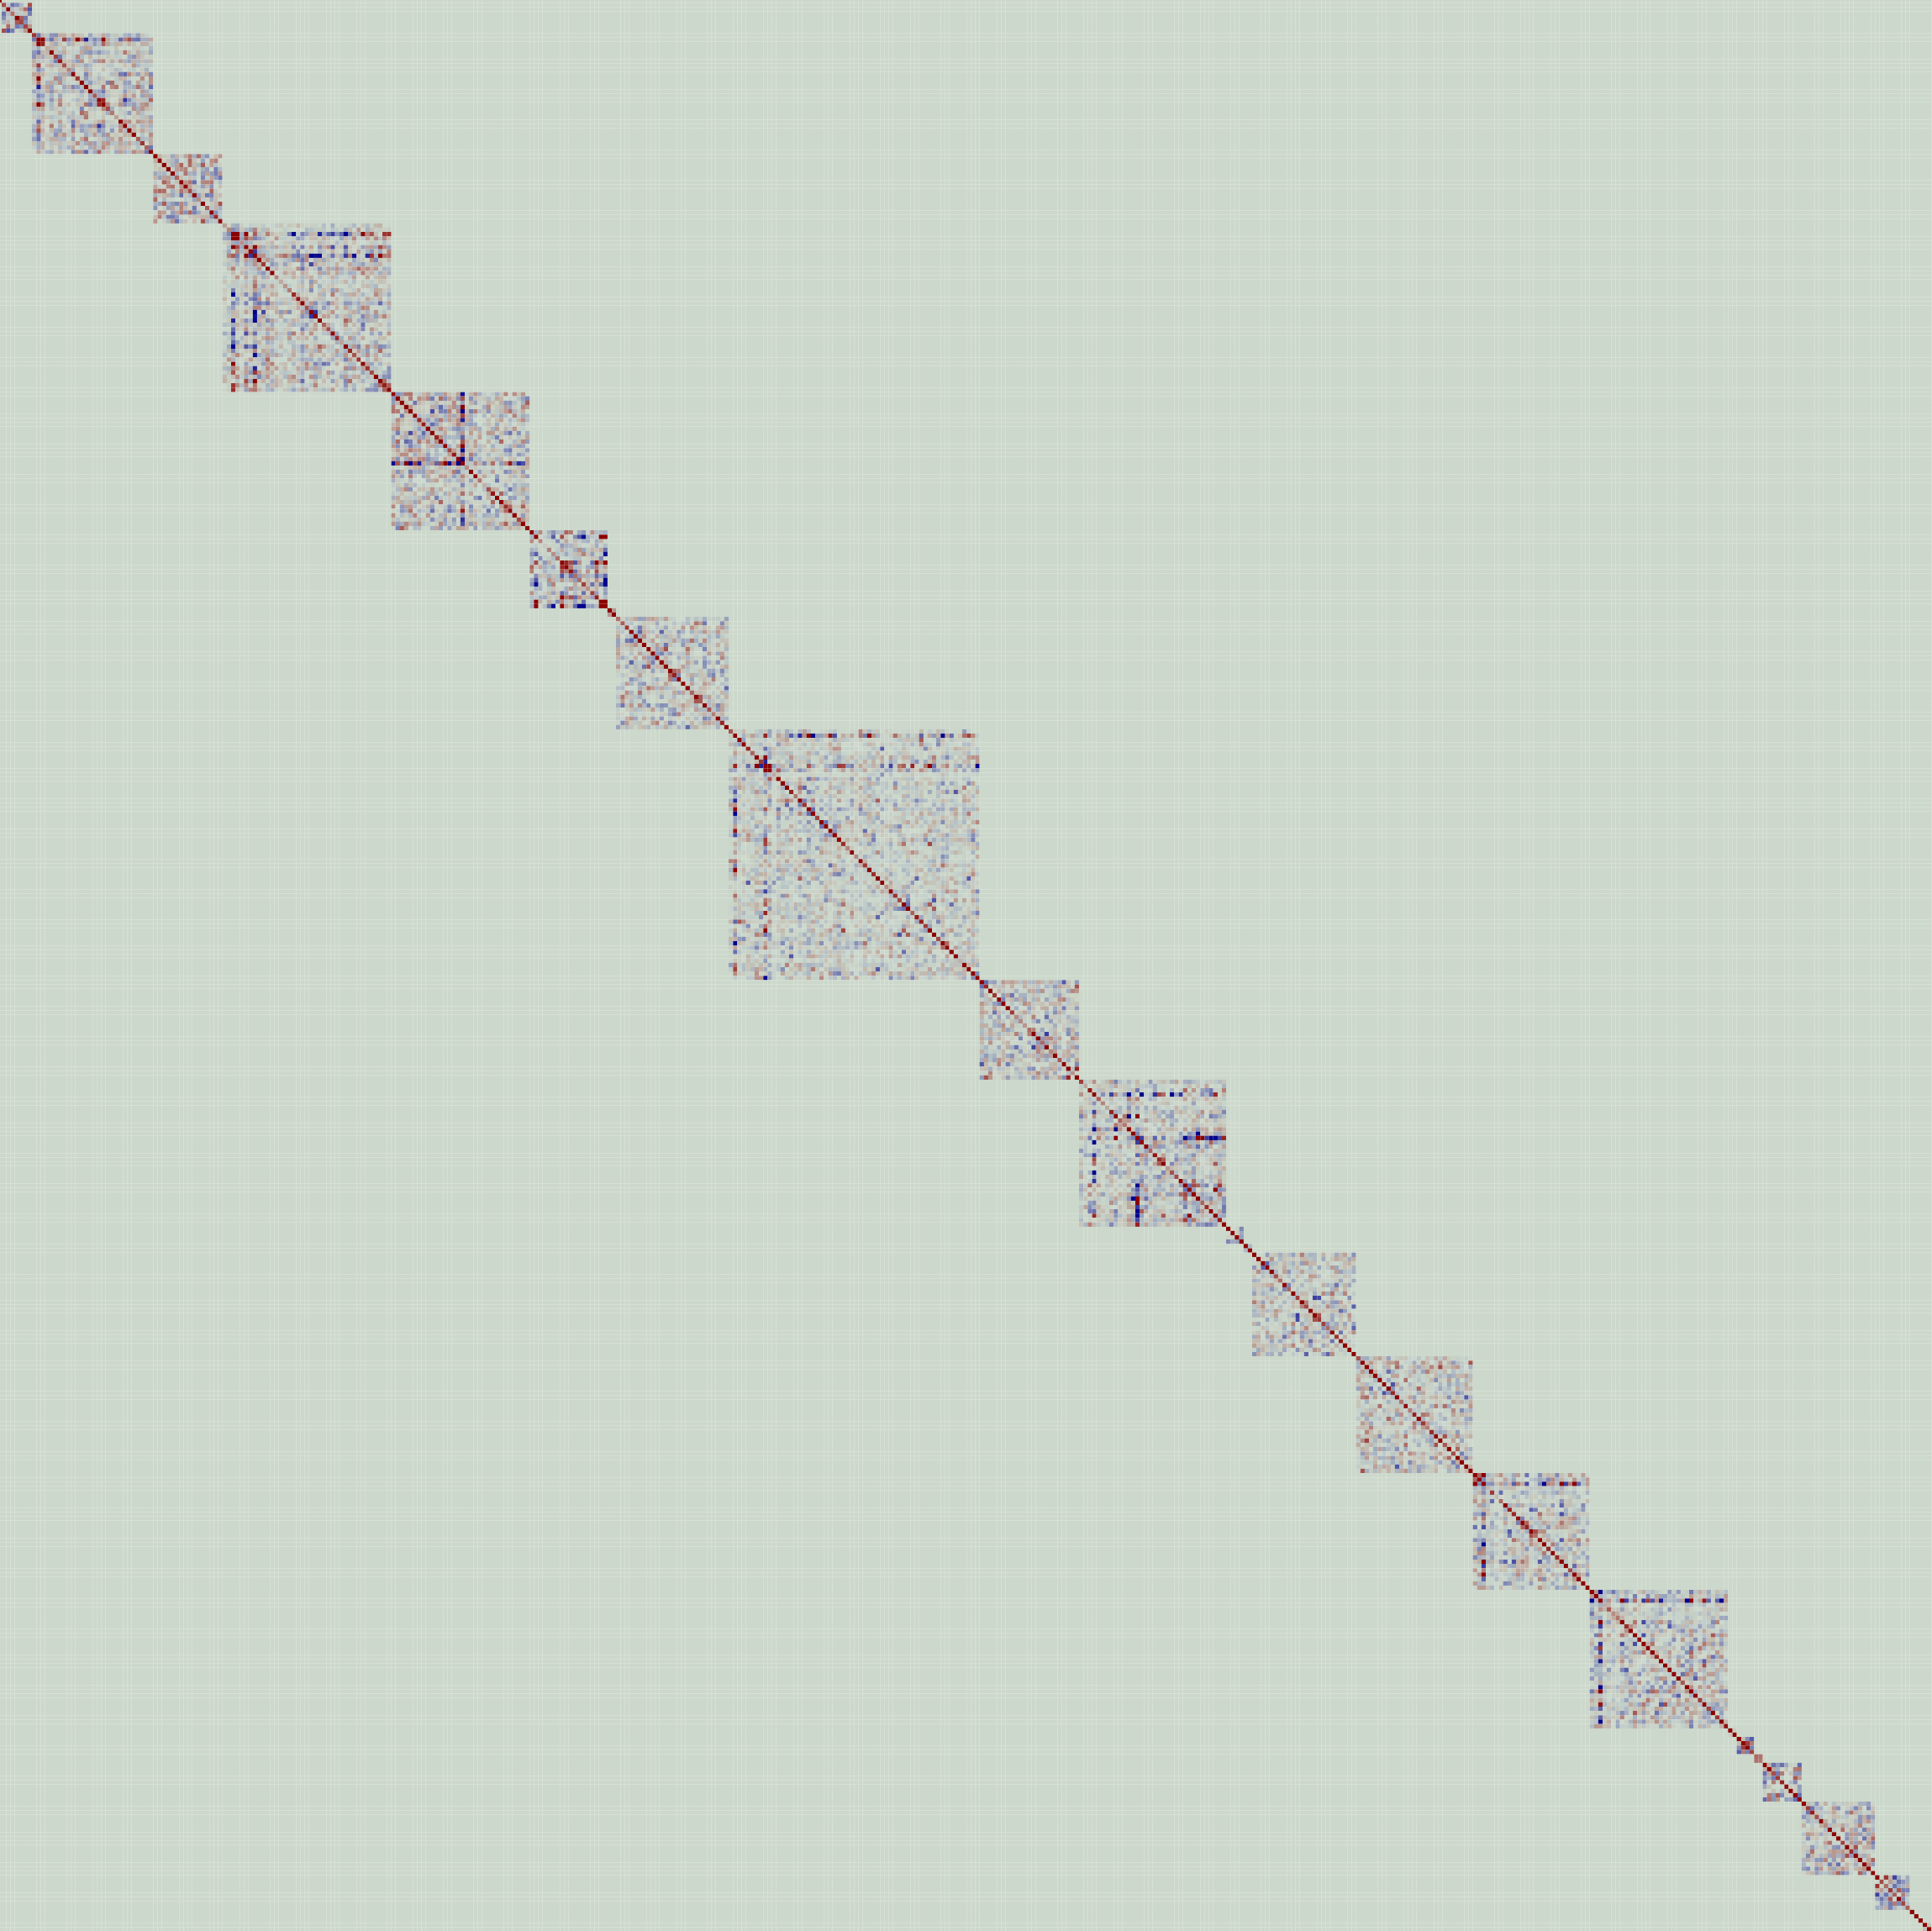
\includegraphics[height=\textheight]{AutF5_blocks.png}
\vfill
\end{center}
\end{frame}

\begin{frame}
\centering
\begin{tikzpicture}[scale=0.9]
\draw [thin, draw=black!20, fill=blue!5] (0,0) grid (10.18,-10.18) rectangle (0,0);
\node at (6.5, -9.5) {Original sdp constraint ($4\, 641 \times 4\, 641$)};
\node (ssdp) at (.5,-.5) {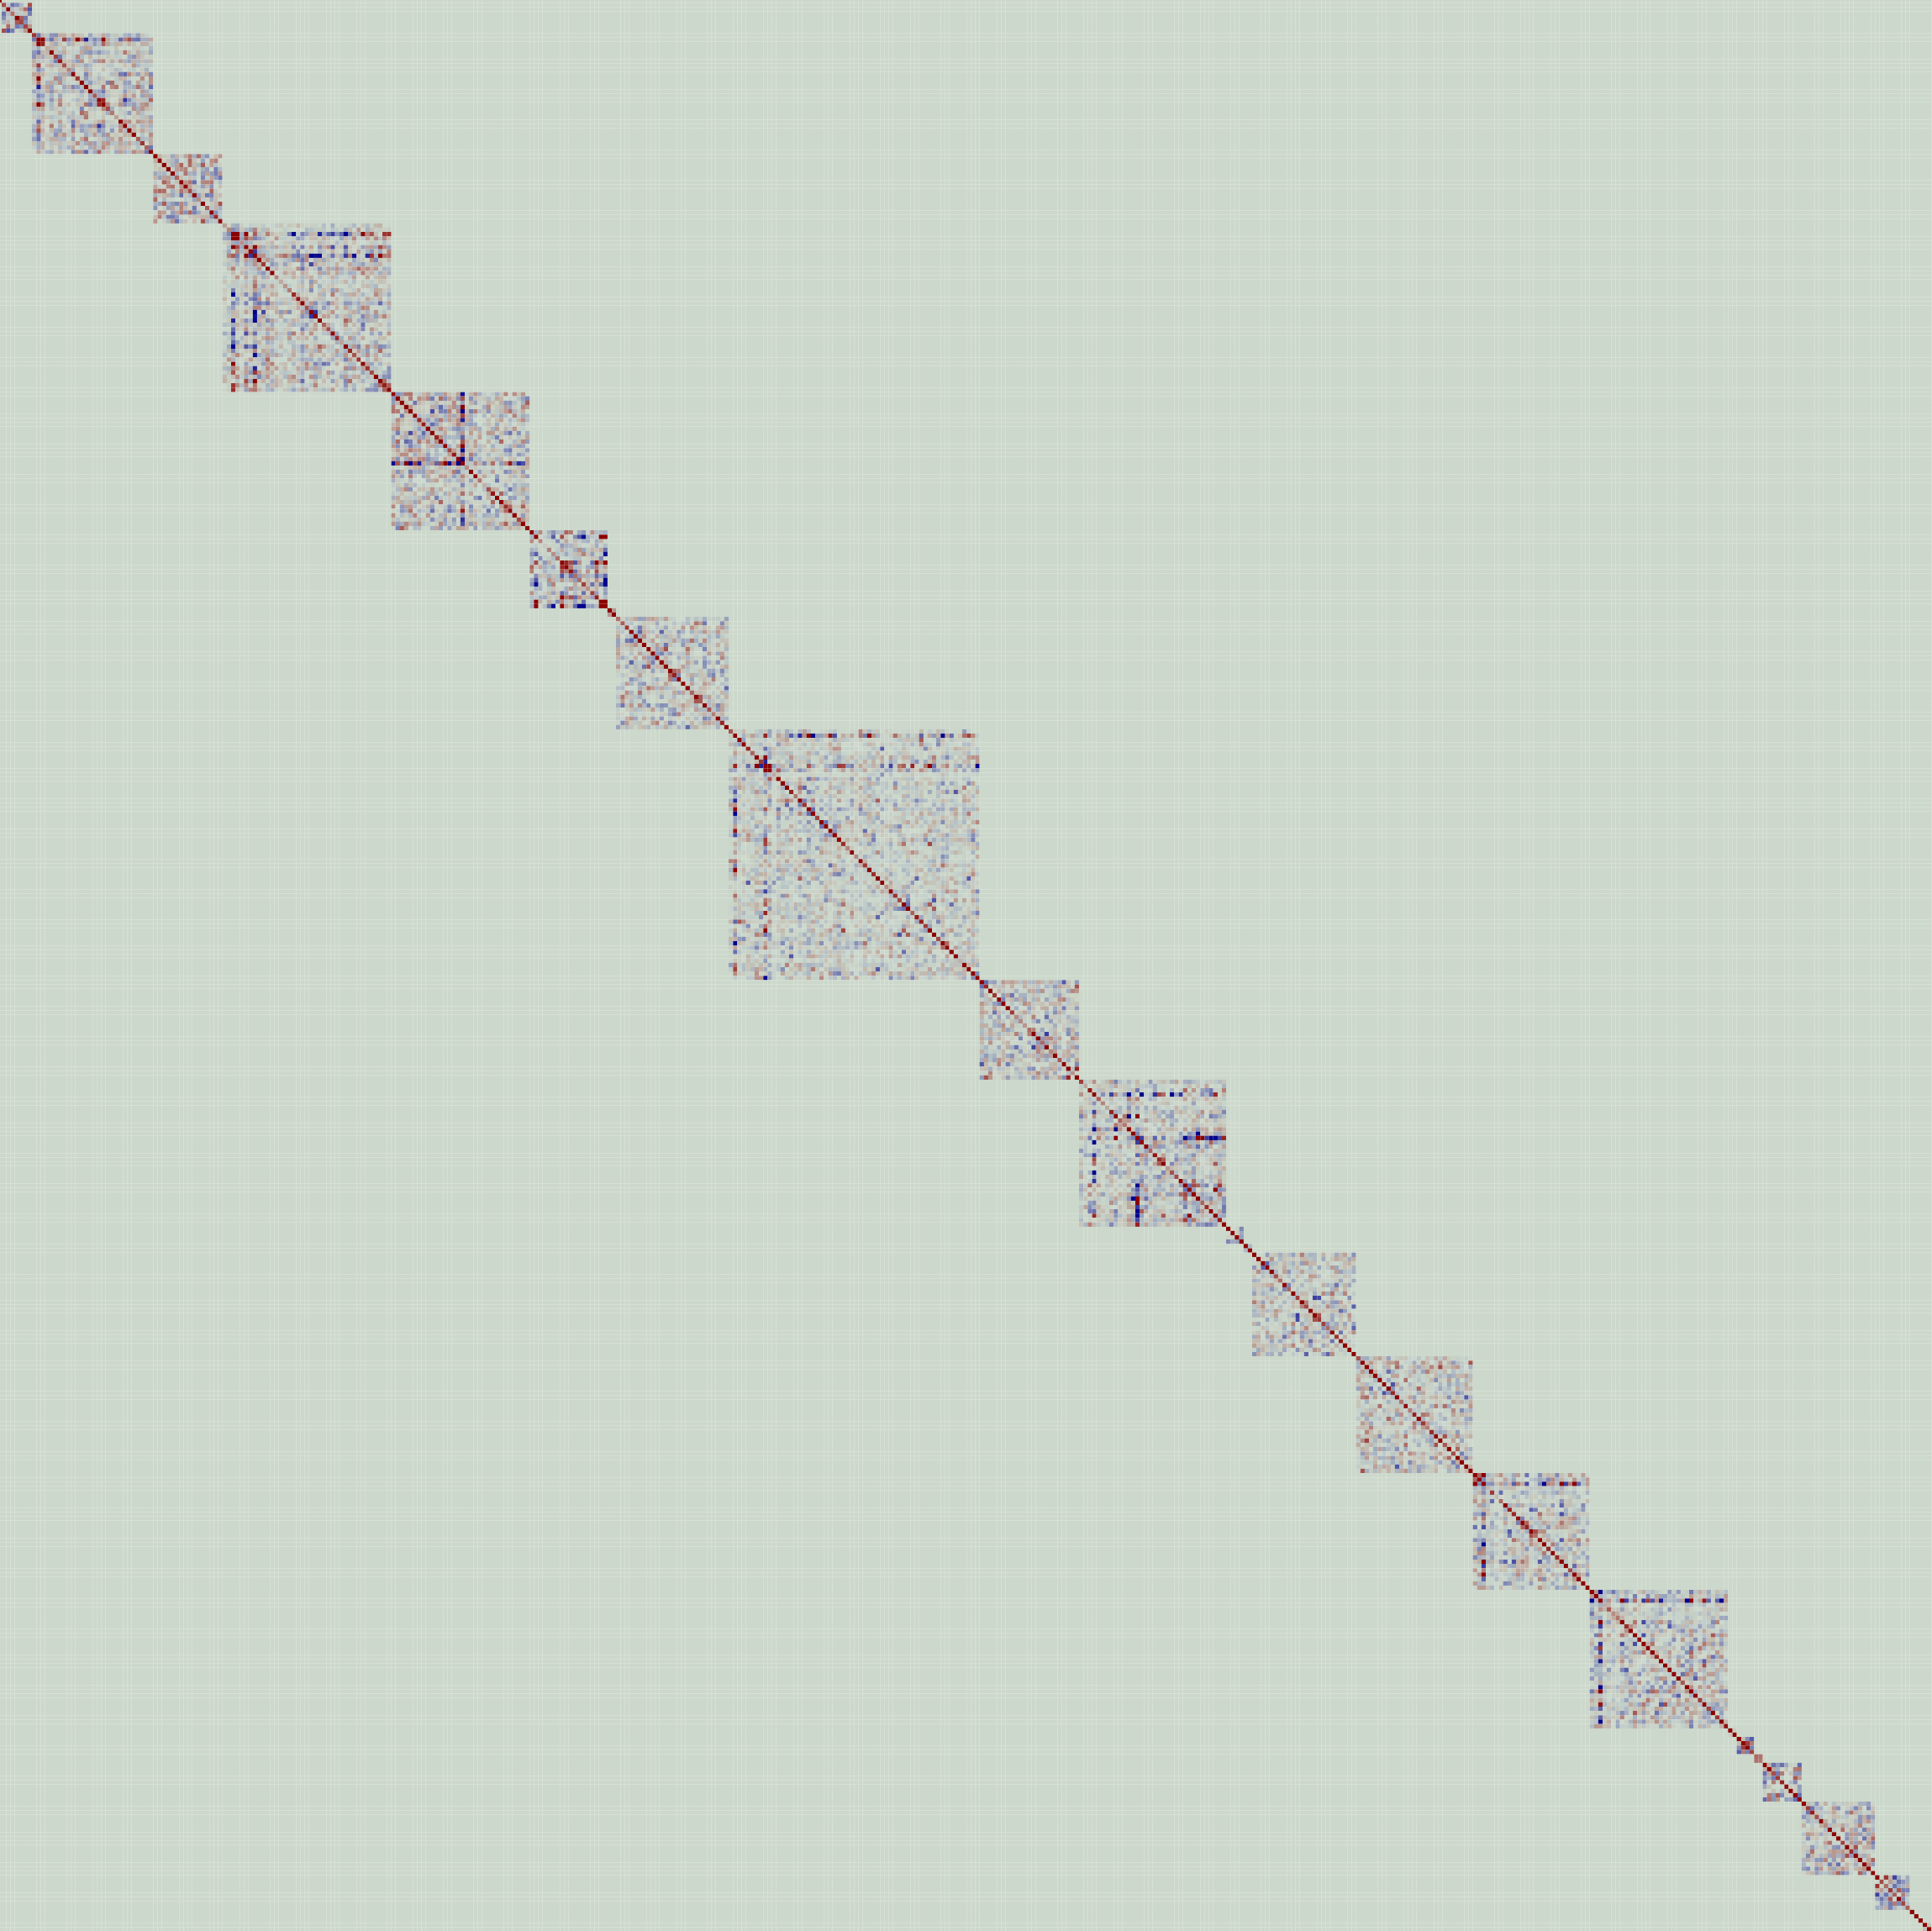
\includegraphics[width=0.9cm]{AutF5_blocks.png}};
\node (label) at (6.5,-.5) {Symmetrized sdp constraint ($448\times 448$)};
\draw [->] (label.west) -- (ssdp.east);
\end{tikzpicture}


\end{frame}






\end{document}
